% sage_latex_guidelines.tex V1.20, 14 January 2017


\documentclass[Afour,times,sagev,doublespace]{sagej}

\usepackage{moreverb,url}

\usepackage[colorlinks,bookmarksopen,bookmarksnumbered,citecolor=red,urlcolor=red]{hyperref}

\newcommand\BibTeX{{\rmfamily B\kern-.05em \textsc{i\kern-.025em b}\kern-.08em
T\kern-.1667em\lower.7ex\hbox{E}\kern-.125emX}}

\def\volumeyear{2019}

\begin{document}

\runninghead{Nugent et al.}

\title{Bias induced by fitting GLMMs with dichotomous outcomes using penalized quasi-likelihood}

\author{Joshua Nugent\affilnum{1}, Bianca Doone\affilnum{1} and Ken Kleinman\affilnum{1}}


\affiliation{\affilnum{1}Department of Biostatistics and Epidemiology,
School of Public Health and Health Sciences,
University of Massachusetts,
Amherst, MA, USA\\}

\corrauth{Ken Kleinman,
Department of Biostatistics and Epidemiology,
School of Public Health and Health Sciences,
University of Massachusetts,
715 North Pleasant Street,
Amherst, MA
01003-9304,
USA}

\email{kkleinman@schoolph.umass.edu}

\begin{abstract}
Generalized linear mixed models (GLMMs) are often used for analyzing data from cluster-randomized trials (CRTs). Popular statistical software packages allow for different GLMM fitting algorithms, but one of these algorithms, penalized quasi-likelihood (PQL), has been shown to produce biased parameter estimates. We review the literature to assess how widely PQL may be used, and conduct a literature-informed simulation study to show the extent of the PQL bias in plausible CRT settings. We find that the algorithms employed are rarely reported in the literature, and that PQL bias is most extreme when the cluster size is small and the variability between clusters is large.

Further, intraclass correlation coefficient (ICC) estimates from PQL-fitted models are also shown to vary by outcome prevalence and treatment effect. Alternatives to PQL estimation are demonstrated to be unbiased and feasible for most CRT data analysis needs.  Analysts should not use PQL and should report fitting methods when reporting trial results.
\end{abstract}

\keywords{Cluster randomized trials, generalized linear mixed models, penalized quasi-likelihood, PQL}

\maketitle

\section{Background}
Generalized linear mixed models (GLMMs) are a commonly used method for analyzing data from cluster randomized trials (CRTs). GLMMs extend generalized linear models (GLMs) by including an additional random-effects term in the linear predictor. This term captures variance between clusters - for example, the group-level differences between hospitals or classrooms. In settings where interventions are applied at the cluster level, GLMMs can disaggregate treatment effects from any underlying variance between clusters. In medical settings, CRTs with dichotomous outcomes are very common - for example, estimating the effect of a new infection control protocol on MRSA incidence, or the probability of a preterm birth for people enrolled in prenatal support groups - and GLMMs are a commonly used tool for analysis. 

The optimization problem of fitting a GLMM to data is a non-trivial task. Two common numerical methods for estimating the coefficients are \textit{penalized quasi-likelihood} (PQL) \cite{wolfinger_generalized_1993} and \textit{Gauss-Hermite quadrature} (GHQ). A third method, the Laplace approximation, is equivalent in this case to a special case of GHQ\cite{liu_note_1994}, so we will simply consider it a subset of GHQ in this paper. Other methods, such as Newton quadrature, Monte Carlo integration, and Markov Chain Monte Carlo can be used as well \cite{zhang_fitting_2011}, but since popular statistical software packages use PQL and GHQ in their standard GLMM fitting algorithms, we will focus on those in this paper. The full mathematical details of these three main methods have been elaborated in other sources \cite{wolfinger_generalized_1993}\cite{pinheiro_efficient_2006}, and an overview of the technical aspects of GLMMs and the algorithms is given in the Supplemental Material.

Penalized quasi-likelihood was popularized by Breslow and Clayton\cite{breslow_approximate_1993}, though similar methods were developed by others\cite{zeger_models_1988}\cite{engel_simple_1994} around the same time. Though it is computationally efficient, especially for models with many random effects, PQL can induce bias in certain cases, in particular when the response variable distribution is far from normal\cite{agresti_categorical_2013}\cite{rodriguez_assessment_1995}\cite{breslow_bias_1995}\cite{lin_bias_1996}. Additionally, PQL produces Wald-type test statistics, not true likelihoods, making it unsuitable for use in the likelihood ratio test. Thus is cannot be used in nested model selection\cite{zhang_fitting_2011}\cite{pinheiro_efficient_2006}\cite{ng_estimation_2006}.

Gauss-Hermite quadrature is a more computationally demanding method, but results in no discernible bias to coefficient estimates, and can produce true likelihood statistics for model comparison. The accuracy with which it computes the model fit is a function of how many \textit{quadrature points} are used. All else being equal, the computation time is roughly proportional to $(N_q)^u$, where $N_q$ is the number of quadrature points and $u$ is the number of random effects at all levels of the model \cite{statacorp_stata_2017}\cite{pinheiro_efficient_2006}. For a model with 4 random effects and 5 quadrature points, $(N_q)^u = 5^4 = 625$. Doubling the number of points to 10 changes that result to $10,000$, a factor of 16. For data sets with large numbers of random effects, this can limit the utility of GHQ.

Luckily for the data analyst, many CRTs have only one random effect, so computation time will increase linearly with the number of quadrature points, rather than as a power function. Furthermore, if many models need to be compared, using one quadrature point can give preliminary results rapidly. Then, after that model selection process, the number of quadrature points can be increased to make the final estimates as accurate as computationally possible. Empirical results suggest that 7 or fewer quadrature points often give suitably accurate estimates\cite{pinheiro_approximations_1995}.

For reasons of computational efficiency, PQL was a useful method when GLMMs were developed, but with the advent of more modern computers, less biased methods such as GHQ have become an attractive alternative. For CRTs with binary outcomes, where the bias in PQL is the most extreme\cite{ng_estimation_2006}\cite{lin_estimation_2007}, and where the presence of only one random effect is typical, using GHQ is the best option: fast enough, and, more importantly, unbiased.

Most modern statistical software packages have functions to fit GLMMs with dichotomous outcomes, such as PROC GLIMMIX in SAS, meglm in Stata, and glmer (from the lme4 package, as well as others) in R. However, the default fitting algorithm in each of those functions varies. In SAS PROC GLIMMIX, the default is PQL, with GHQ available if specified. In R, the glmer function default is GHQ with a single quadrature point, with more points possible if specified; PQL is only available in R via the glmmPQL function in the MASS package. In Stata, meglm defaults to GHQ with 7 quadrature points; PQL is not an option. In SPSS, PQL is the default, with no option to use GHQ.

Given that many data analysts may be unfamiliar with the fitting options, a function's default settings are influential in the final results. Below, we investigate how often functions and algorithms are reported in the literature and use simulations to describe the bias induced by PQL in a literature-informed, plausible CRT scenario.


\section{Methods}


We started by conducting a literature review among recent CRTs with dichotomous outcomes to determine a) common values for cluster size and number of clusters and b) what software, functions, and fitting algorithms were used to analyze the data, if reported. In this review, we searched for the phrase "cluster randomized trial" in the title or abstract of all articles in the PubMed database published between March 1st, 2018 and August 31, 2018. Having identified candidate articles, we filtered to completed CRTs with dichotomous outcomes. The mean number of observations per cluster and number of clusters for each study was recorded, as well as the software and functions/algorithms the authors used, if available.

The second phase of our work was a simulation study to investigate the bias of different GLMM fitting algorithms for dichotomous outcomes. To maximize the utility of the results, our simulations used a range of plausible cluster counts and cluster sizes drawn from the literature review.

The data-generating mechanism for the simulations was a simple logistic-link GLMM with a fixed intercept, treatment effect, and one random intercept:

\begin{equation}
    \text{logit}[\text{Pr}(y_{ij}|b_j)=1]=\beta_0 + \beta_1 x_{ij} + b_j
\end{equation}

with $x_{ij}$ an indicator for treatment (1) or control (0) arm of the study for unit $i$ in cluster $j$; $\text{Pr}(y_{ij}|b_j)$ the probability of the outcome $y$ for unit $i$ in cluster $j$; $\beta_0$ the log odds of the outcome for the mean cluster in the control arm; random intercept $b_j$ with assumed distribution $b_j \sim N(0, \sigma^2)$; and $\beta_1$, our parameter of interest, the log odds ratio due to the treatment. 

From that model, populations were generated with the following parameter values, informed by the literature review:
\begin{itemize}
    \item Number of clusters $\in \{20, 50, 100\}$
    \item Number of observations per cluster $\in \{25, 100\}$
    \item $\beta_0$ values corresponding to a baseline prevalence of .02, .03, and .2
    \item $\beta_1$ values corresponding to a treatment effect odds ratio of 1.1, 1.33, 1.5, and 2
    \item $\sigma^2$ values of .1 (low between-cluster variability), and 1 (high between-cluster variability); for the data sets with 25 observations per cluster, we also examined $\sigma^2=.25$ and $.5$.
\end{itemize}

Using 5000 simulated datasets for each combination of parameters, logistic-link GLMMs were fit via PQL and GHQ using SAS/STAT software version 15.1 (SAS Institute Inc., Cary, NC).

The distribution of $\hat{\beta}_1$ estimates from each method was compared to the true value from the data-generating mechanism and absolute bias was measured as the difference between the two. The standard errors of estimates and the estimated cluster variance ($\hat{\sigma}^2$) were also collected from the fitted models, and model-fitting CPU time was measured. Finally, the simulated populations were re-fit under the assumption that the outcome variable was normally distributed, without the logit link, and the intraclass correlation coefficient (ICC) estimated from those models was collected.

A small number of datasets with small cluster sizes resulted in zero events in one arm; in this case the estimates of $\beta_1$ will tend toward infinity, so these datasets were excluded from the analysis.

To test the speed of the algorithms, we calculated the mean CPU time for SAS and R to fit large data sets of 500 clusters and 500 observations per cluster using the different methods.





\section{Results}

The literature review identified 43 candidate articles. Among them, only 4 identified the specific procedure used (meglm in Stata or PROC GLIMMIX in SAS, for example). Among the 11 articles that identified SAS as one of the software packages, only 2 specified which SAS procedure was used and none identified the model fitting algorithm. Ten articles did not report the software used at all.

Parameters for the simulations were chosen after observing the common values in the literature review. The median number of clusters was 32, with the middle 50\% between 17 and 70. The number of observations per cluster showed more variability, with a median of 44 and the middle 50\% between 14 and 205.

\begin{figure}
\centering
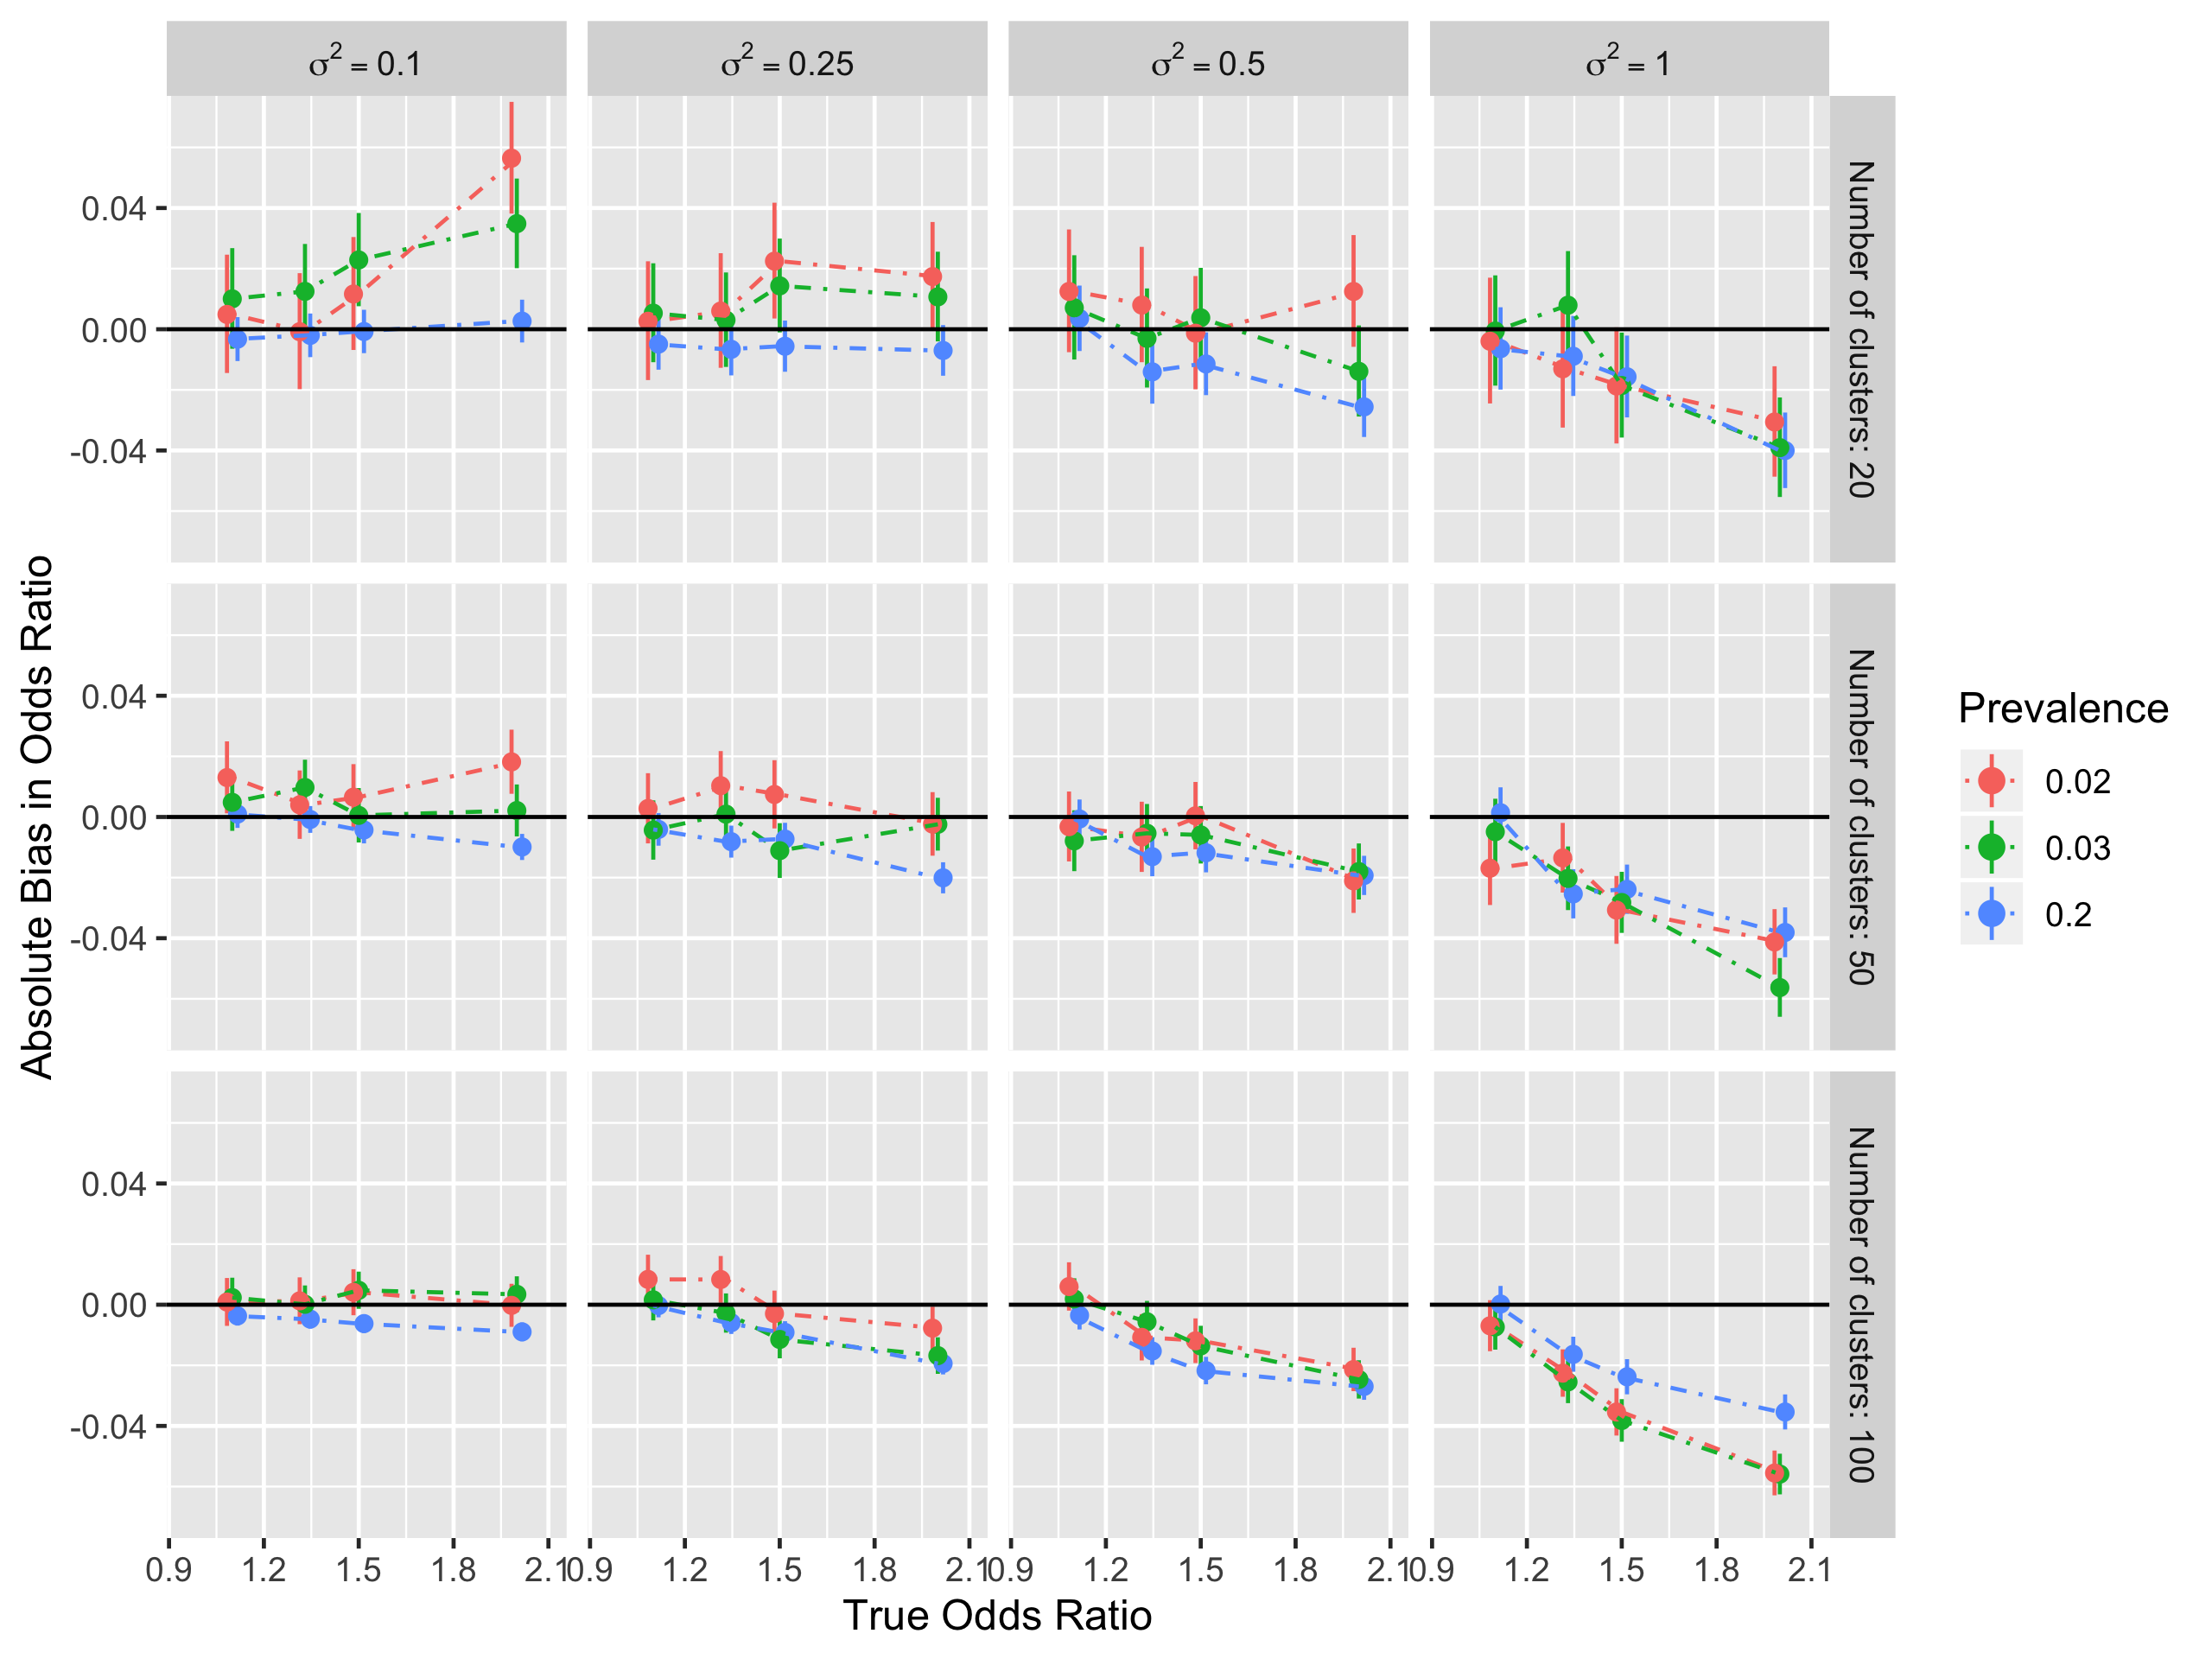
\includegraphics[width=\linewidth]{_bias_pql_all_sbs.png}
  \caption{Odds ratio bias ($\text{exp} \{ \bar{\hat{\beta_1}} - \beta_1 \} - 1$) in PQL estimation, 25 observations per cluster.}
    \label{fig:_bias_pql_all_sbs_p25}
\end{figure}


\begin{figure}
\centering
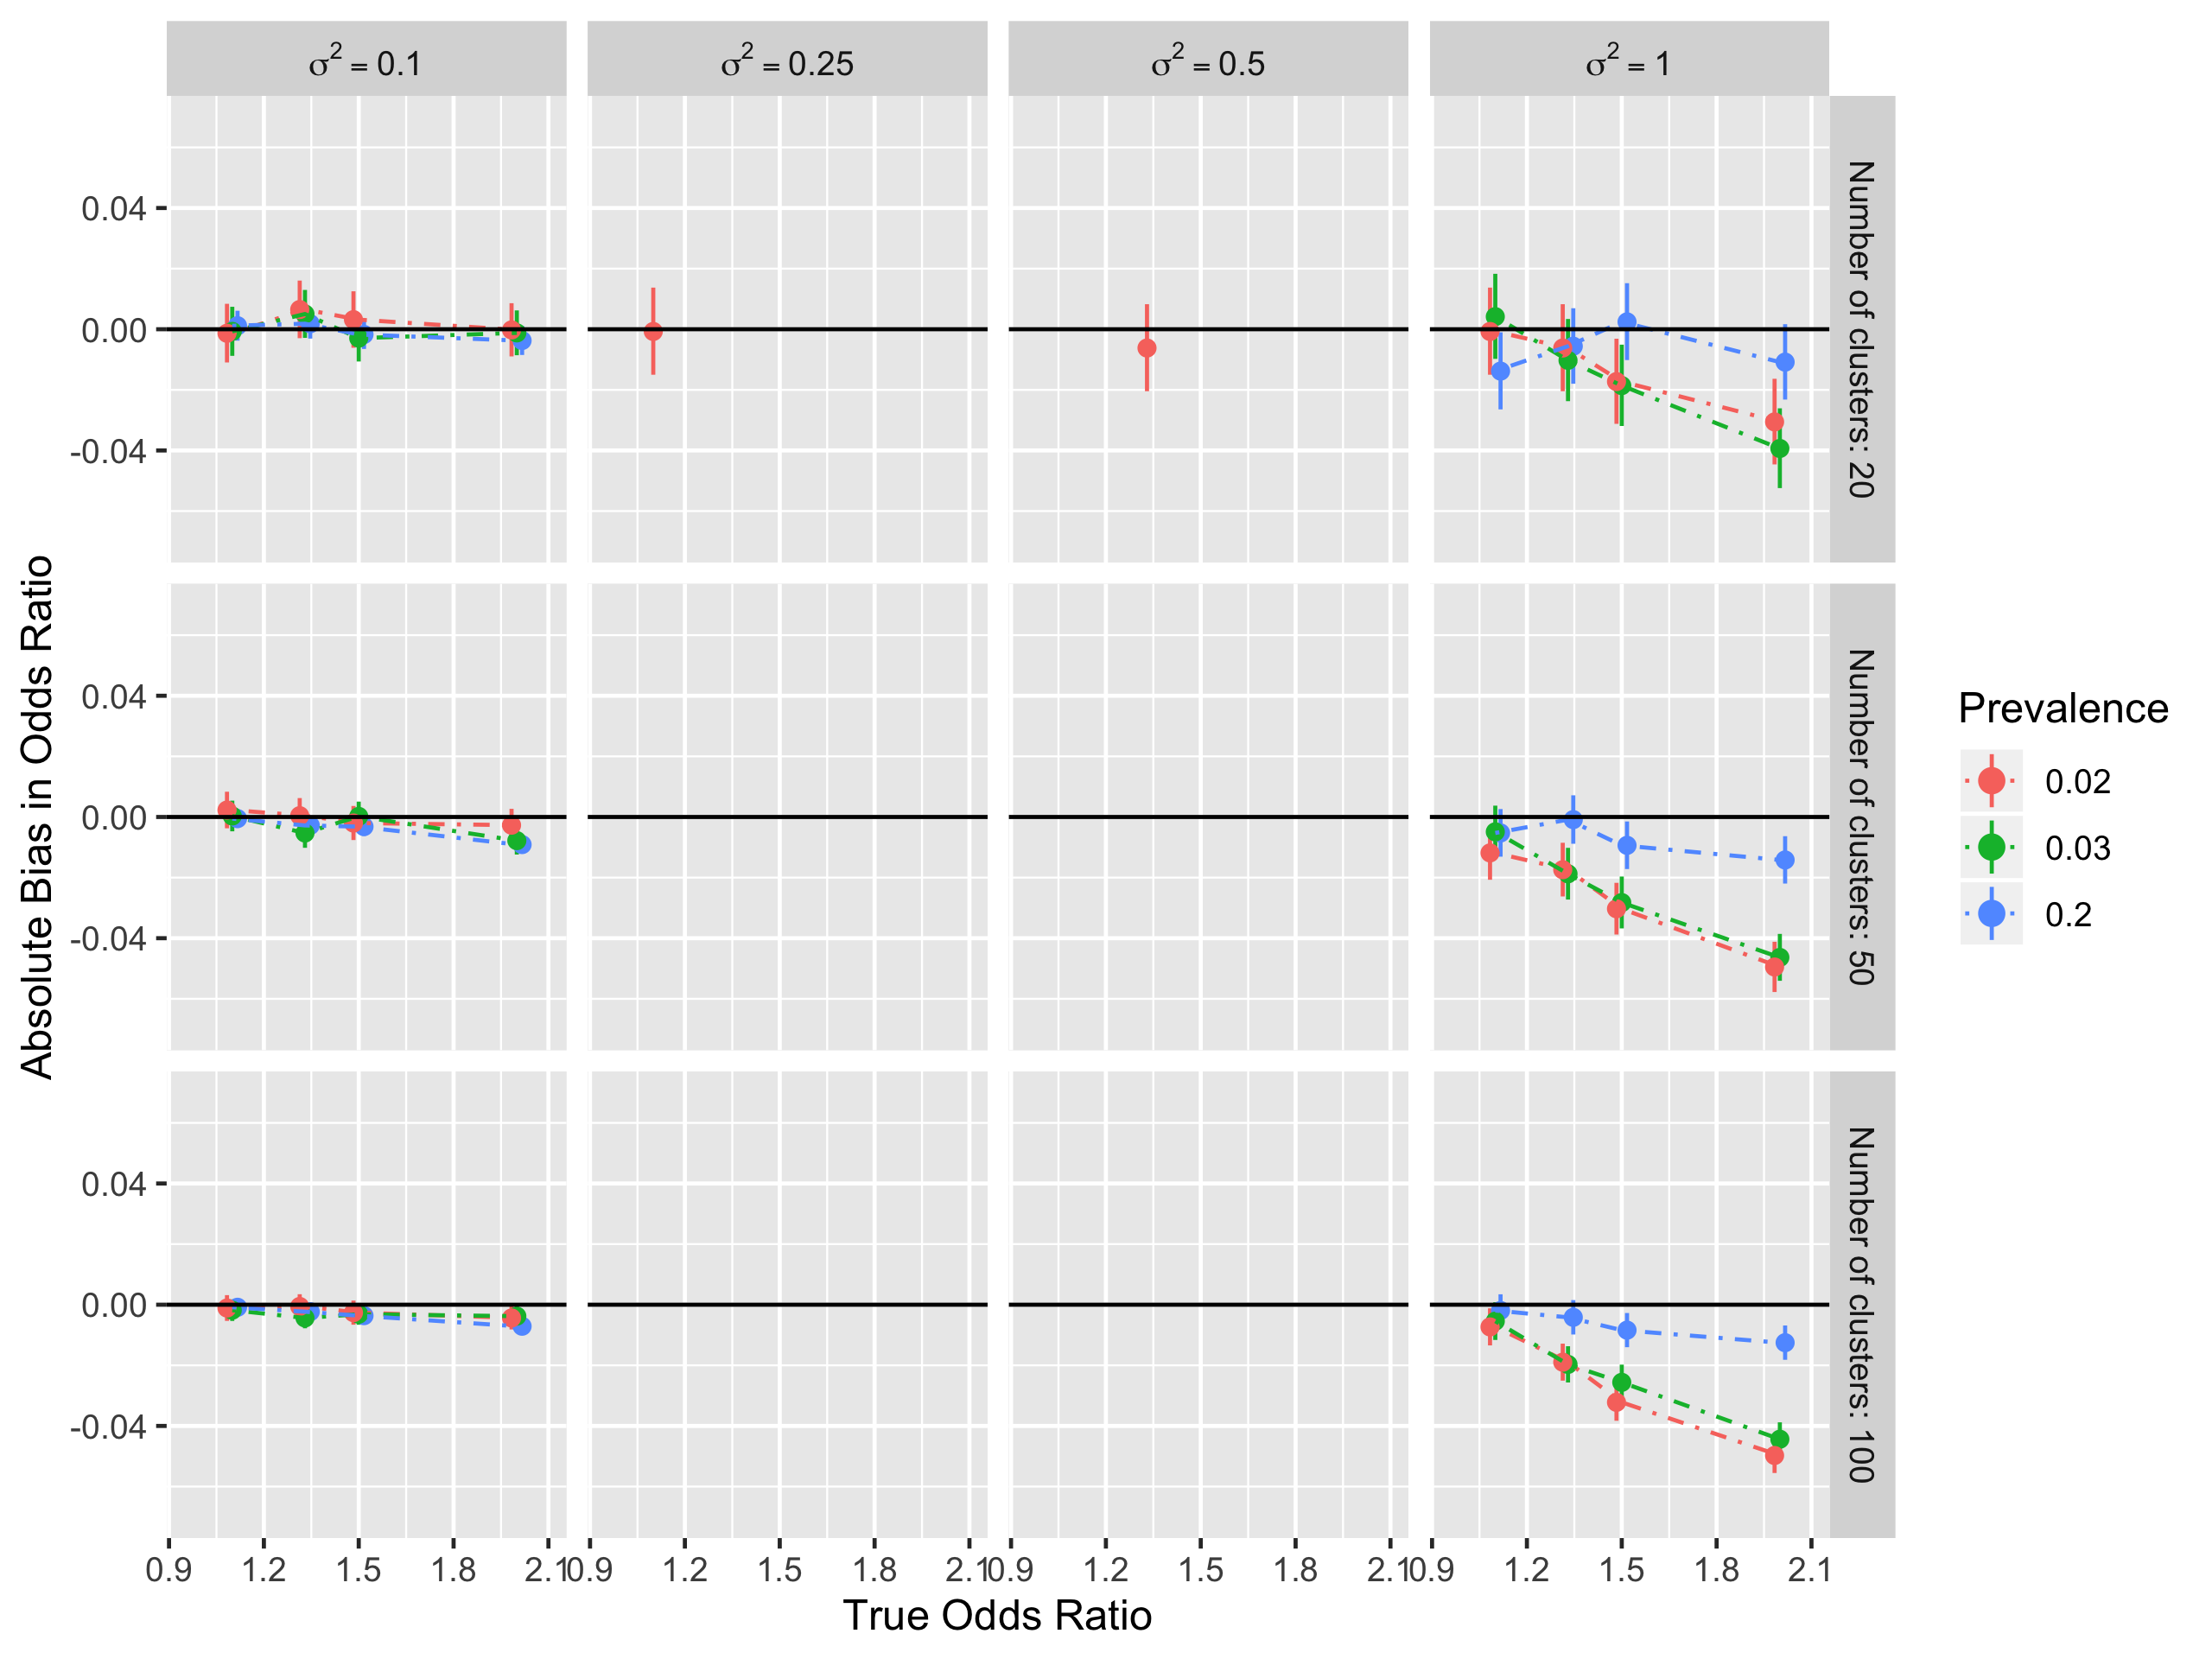
\includegraphics[width=\linewidth]{_bias_pql_all_sbsP100_temp.png}
  \caption{Odds ratio bias ($\text{exp} \{ \bar{\hat{\beta_1}} - \beta_1 \} - 1$) in PQL estimation, 100 observations per cluster.}
    \label{fig:_bias_pql_all_sbs_p100}
\end{figure}


The results of the bias investigation in PQL estimation are shown in Figures \ref{fig:_bias_pql_all_sbs_p25}-\ref{fig:_bias_pql_all_sbs_p100}. When $\sigma^2$ is large, there is a bias towards the null: As the true odds ratio rises above 1, there is a negative bias, meaning the mean estimated odds ratio is closer to 1 than it should be. In these cases with a large $\sigma^2$, the bias is slightly more pronounced for smaller cluster sizes when the outcome's baseline prevalence is low. A large number of clusters leads to the most extreme negative bias, holding all other factors constant.

As $\sigma^2$ becomes smaller, the negative bias is diminished, holding other factors constant. In fact, it can even become noticaebly positive when the clusters are small, the outcome prevalence low, there are a relatively small number of clusters, and the between-cluster variability is small, as shown in Figure \ref{fig:_bias_pql_all_sbs_p25}. In these cases, the pattern reverses, and there is a bias away from the null.

The fitted models using GHQ (a representative example is given in Figure \ref{fig:_bias_pql_ghq4}) did not show a clear bias; PQL is shown for reference.

\begin{figure}
\centering
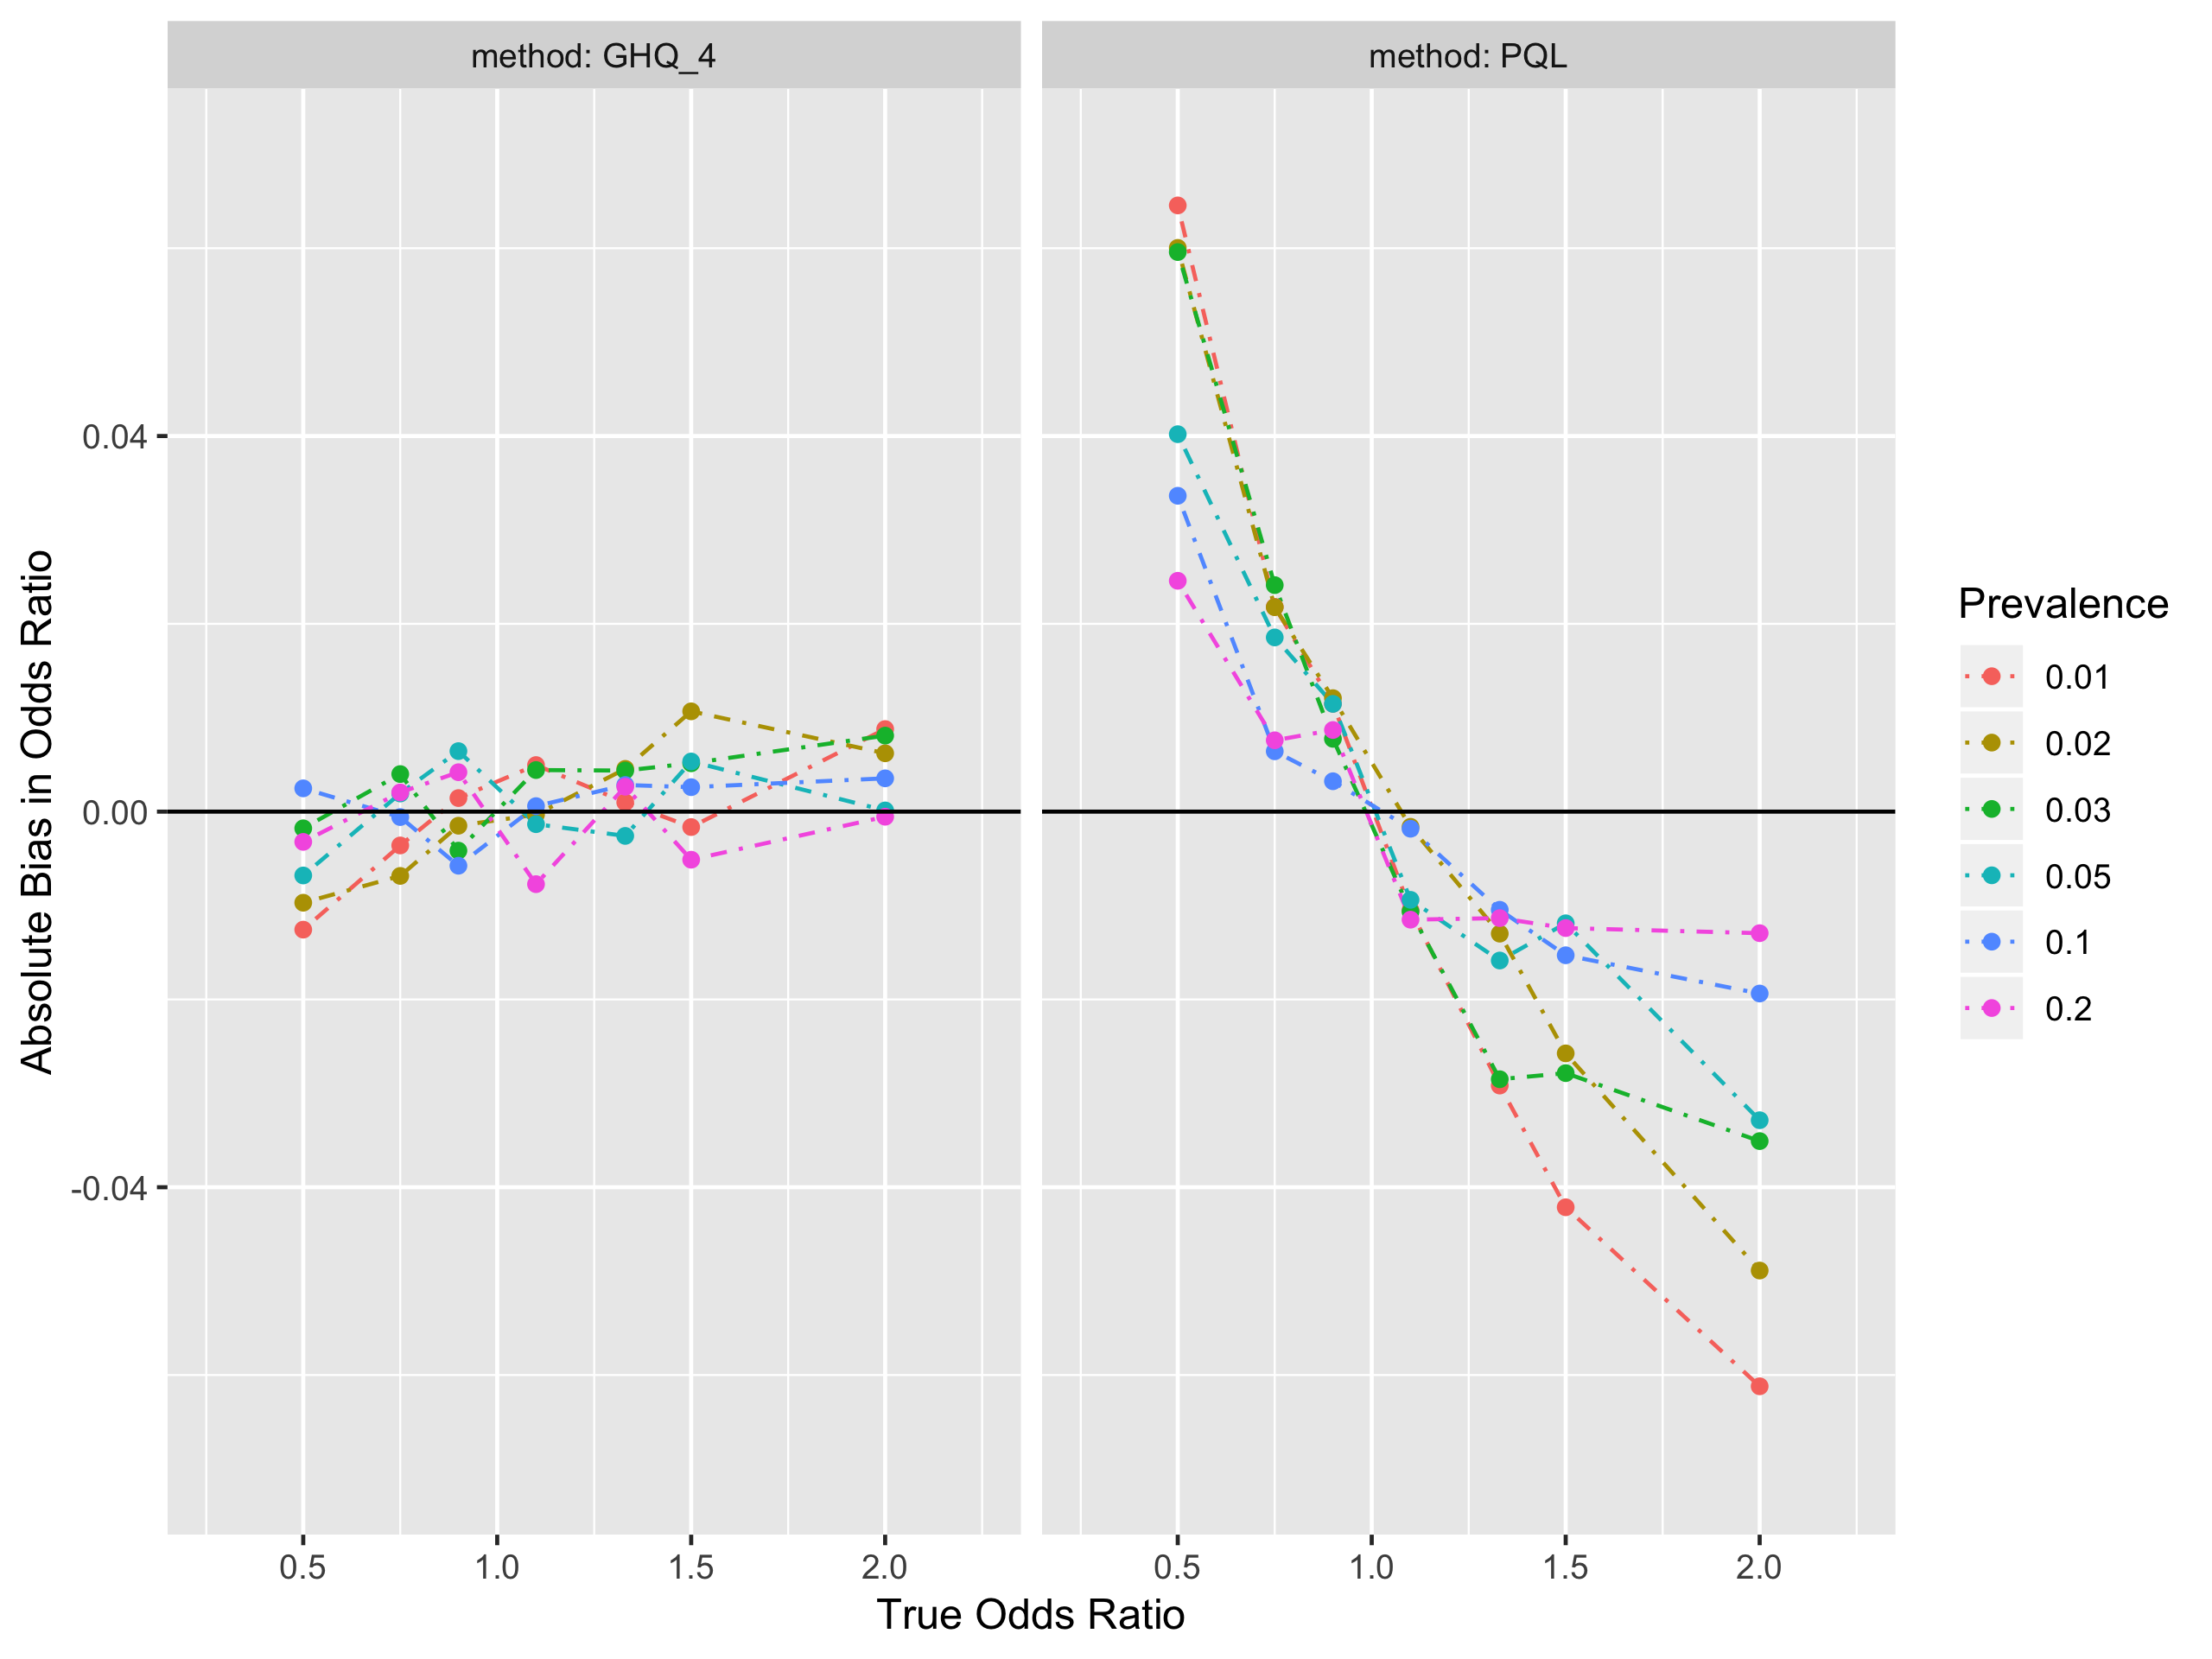
\includegraphics[width=\linewidth]{_bias_pql_ghq4.png}
  \caption{Odds ratio bias ($\text{exp} \{ \bar{\hat{\beta_1}} - \beta_1 \} - 1$) in GHQ (4 quadrature points) and PQL, $\sigma^2=1$, 100 units/cluster, 100 clusters.}
  \label{fig:_bias_pql_ghq4}
\end{figure}

Our simulations confirmed that the main advantage of using PQL over GHQ is speed, shown in Table \ref{tab:method_speed}. SAS's implementation of PQL outperforms the other methods, and is much faster than the glmmPQL method in the MASS package for R. Results for GHQ are similar for both SAS and the lme4 package in R.


\begin{table}[h]
\centering
 \begin{tabular}{l | c c} 
 Method & R & SAS \\ 
 \hline
 PQL & 23.3 & 3.7 \\ 
 GHQ (4 quadrature points) & 16.1 &  18.4 \\
 GHQ (10 quadrature points) & 22.0 &  27.1 \\ 
 \end{tabular}
    \caption{Mean time in seconds to fit a data set with 500 observations per cluster and 500 clusters.}
    \label{tab:method_speed}
\end{table}

Though it is not an actual parameter of the model, data analysts may be interested in the intraclass correlation coefficient (ICC). In normally distributed data, the ICC measures the proportion of total variance that is explained by the variance between groups. However, in the case of a non-normally distributed outcome variable, there has been considerable discussion about how to appropriately characterize and calculate the ICC\cite{wu_comparison_2012}\cite{nakagawa_shinichi_coefficient_2017}. We generated two ICC estimates using the PQL-fitted models from our simulation.  First, a version that assumed a random intercept logistic model, implying an ICC of $\frac{\sigma^2}{\sigma^2+\frac{\pi^2}{3}}$, based on the estimated between-cluster variance\cite{wu_comparison_2012}. Second, a linear mixed model was fit using SAS PROC MIXED that assumed the outcome variable was normally distributed, leading to the ANOVA-based calculation $\frac{\sigma^2}{\sigma^2+\sigma^2_{\epsilon}}$, where $\sigma^2_{\epsilon}$ represents the variance of the residuals\cite{wu_comparison_2012}. The results are shown in Figure \ref{fig:_icc} for two values of $\sigma^2$ examined in the simulations. In both cases, the estimated ICC varies by prevalence, treatment effect, and ICC calculation method.

\begin{figure}[]
\centering
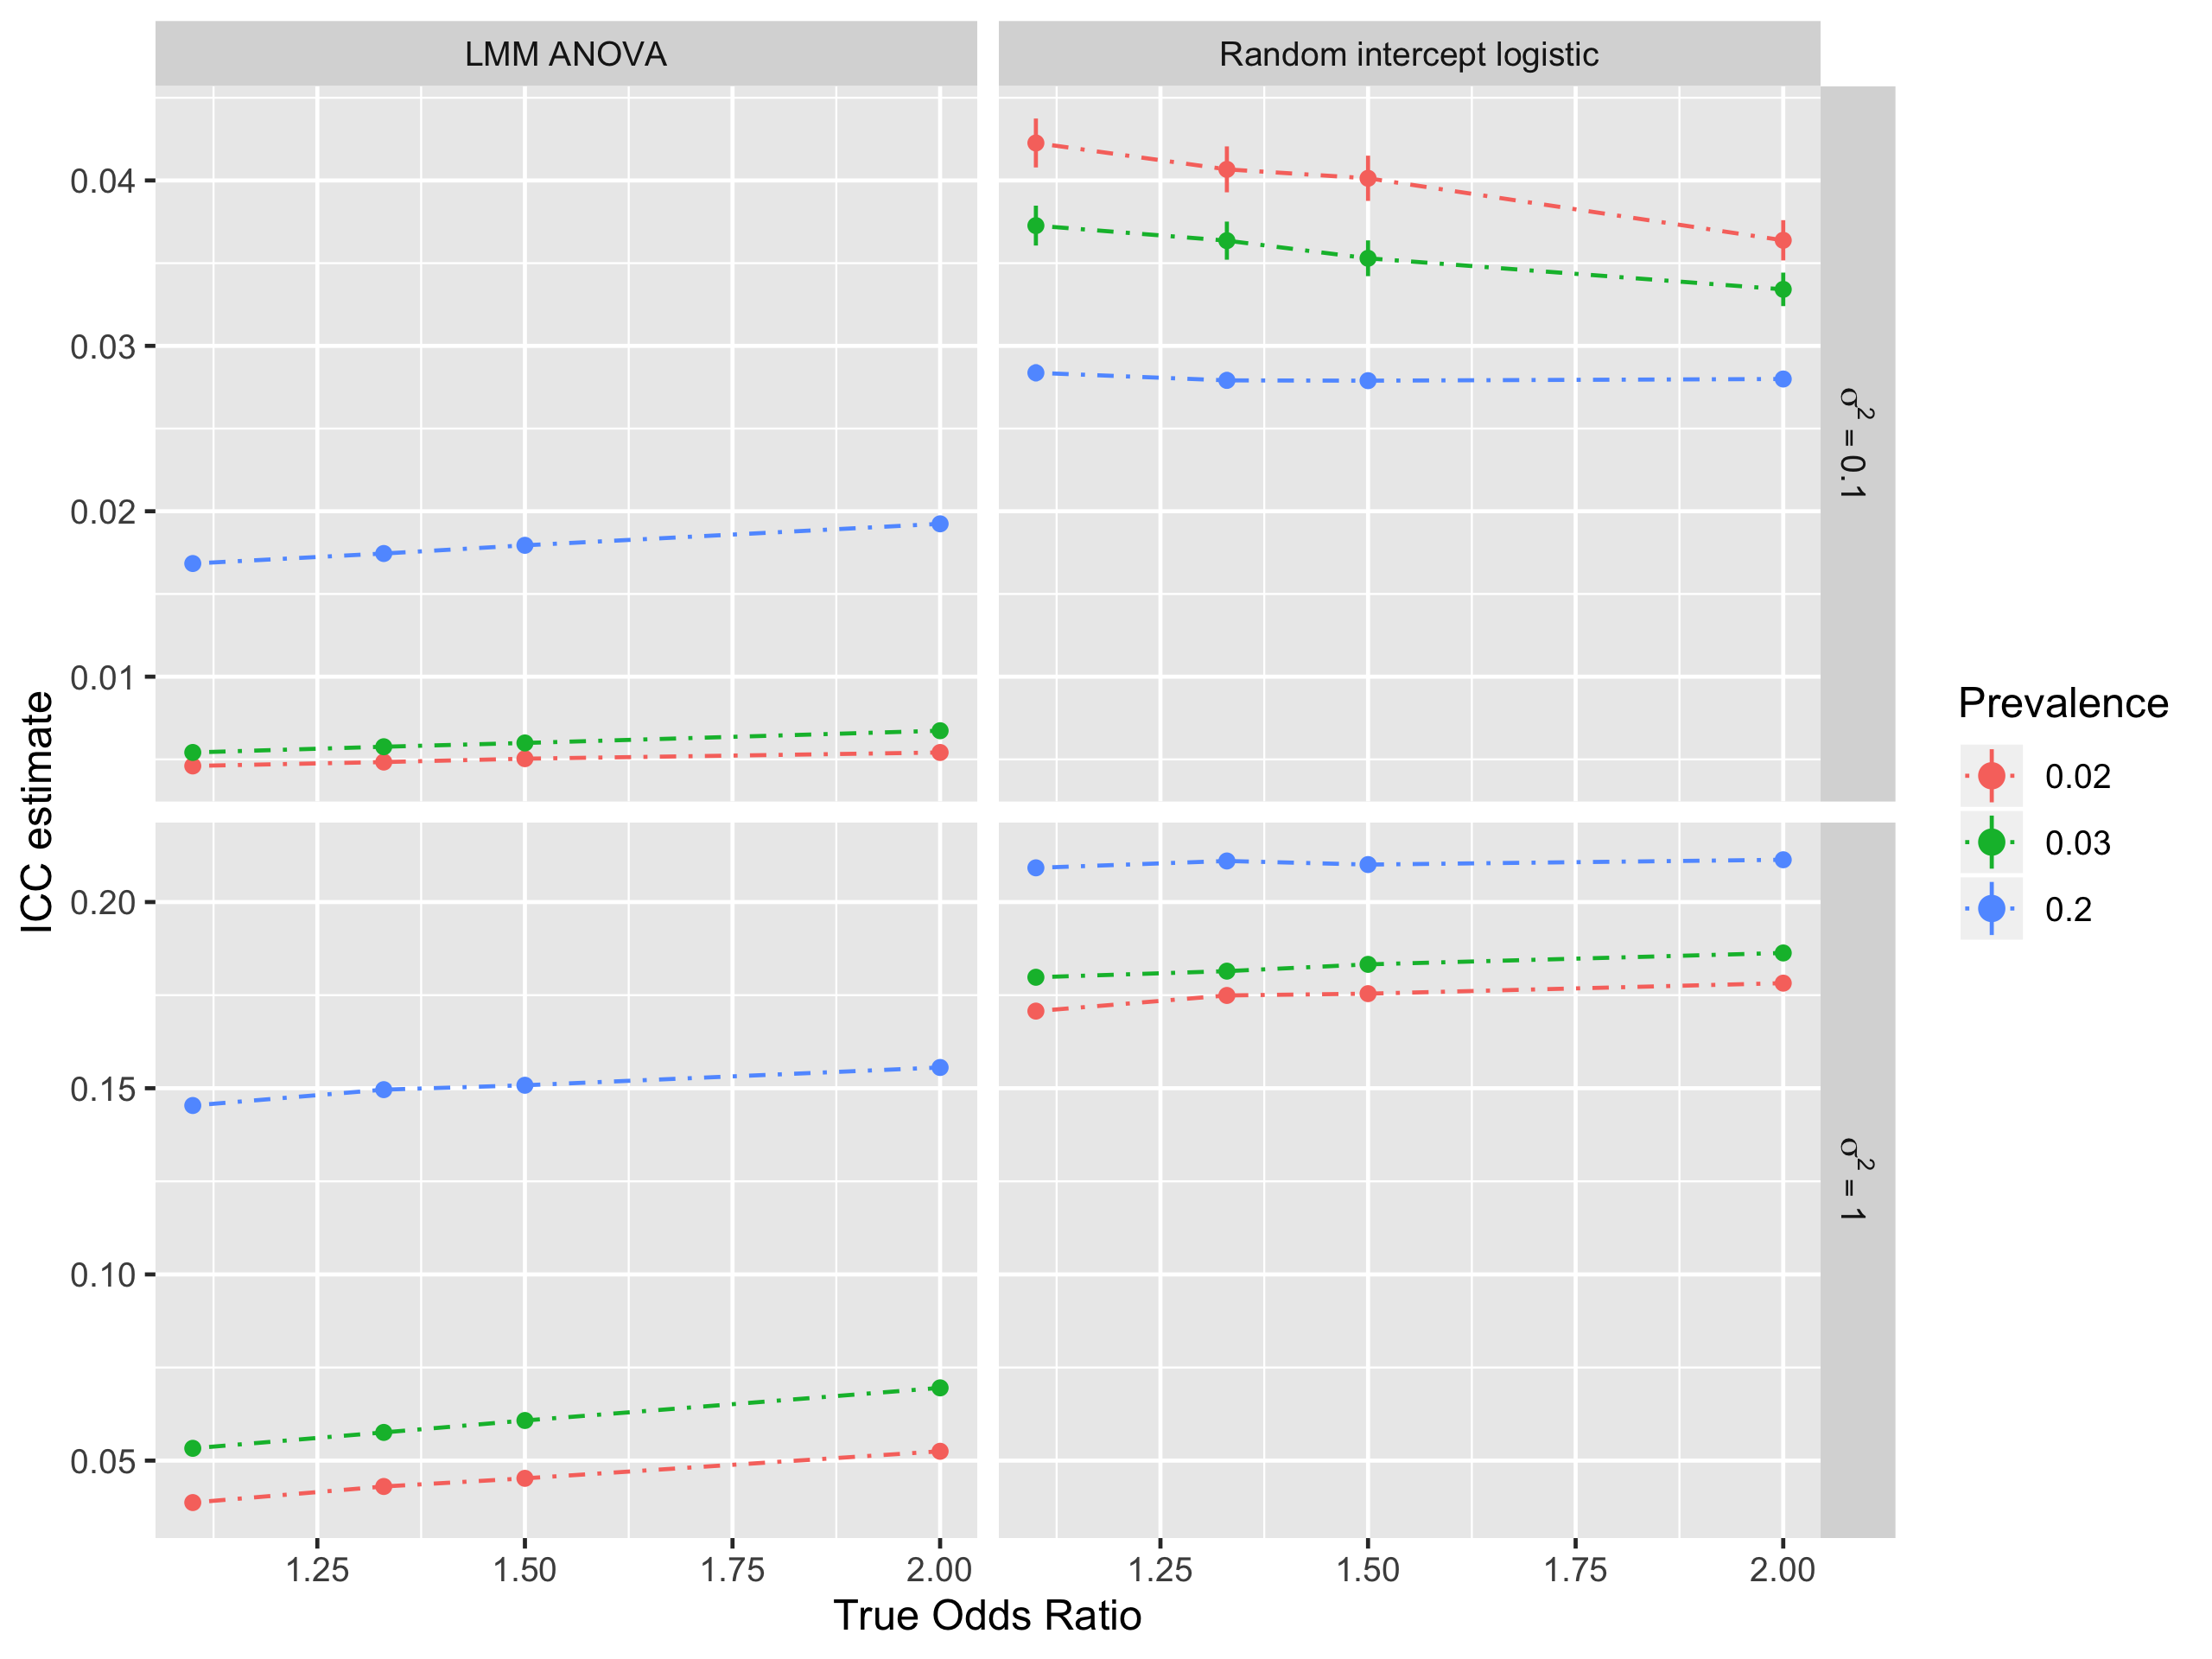
\includegraphics[width=\linewidth]{_icc_p25_n50v2.png}
  \caption{ICC estimates, 25 observations per cluster, 50 clusters.}
    \label{fig:_icc}
\end{figure}


\section{Discussion}

For CRTs with sample sizes that occurr commonly in the literature, using PQL to estimate coefficients in random intercept logistic regression shows a noticeable bias, particularly if the true odds ratio is far from 1. GHQ, on the other hand, shows no noteiceable bias, so for the vast majority of cluster randomized trials with dichotomous outcomes, GHQ is superior to PQL when fitting models. To fit a single data set with a small number of random effects, and given than most CRTs have only one random effect, the speed of GHQ with 4-10 quadrature points is adequate and it produces no detectable bias.

We note that data analysts experimenting with different nested models can use GHQ with a single quadrature point during the model-selection stage to save time, then larger number of points once the final model has been chosen. GHQ is also preferable to PQL in the model-selection process because PQL only provides quasi-likelihood, and hence it is not suited to nested model comparison with the likelihood ratio test. However, model selection is not usually a task in CRT analysis.

The bias towards the null generated by PQL is more pronounced when clusters are small, between-cluster variance is high, baseline incidence of an outcome is low, and the number of clusters is large. Bias away from the null may arise when the number of clusters, the cluster size, and the between-cluster variance is small. Given our simulations, we suspect that existing studies may have suffered this bias, though it is hard to be sure given that fitting methods are rarely reported in the literature. Trial reports should include methods/functions and the algorithm options in more detail.  We should take care when selecting procedures for fitting GLMMs, particularly in SAS and SPSS, where PQL is the default option.

Previous work investigating PQL estimation in scenarios with dichotomous outcomes has noted the bias\cite{jang_numerical_2009,zhang_fitting_2011}, but not examined the full interactions between cluster size, number of clusters, baseline prevalence, true odds ratio, and cluster-level variance as have here. We hope this will make it easy for analysts to identify situations where bias could be present.

Given the bias it creates, why use PQL? As noted above, PQL fits models much more quickly than GHQ. However, our simulations showed that even for large data sets, none of the runtimes are prohibitively long, given a typical CRT model with one random intercept term. In a situation where many models need to be tested, a single quadrature point could be used to compare models, and then for the final analysis, a more accurate fit could be made with a large number of quadrature points.

Finally, ICC estimates generated by these algorithms may vary substantially by the method used to calculate them and by the baseline prevalence of the outcome, and should be approached with a degree of caution.







\begin{funding}
Grant Support: NIGMS: R01 GM121370
\end{funding}

\begin{sm}

\subsection{GLMM Fitting}
Mathematically, a GLMM can be modeled as
    \begin{equation}
        g(\mu_{it})=\mathbf{x}^T_{it} \boldsymbol{\beta} + \mathbf{z}^T_{it}\mathbf{u}_i
    \end{equation}
    
    with
 $i$ a cluster indicator, $t$ an observation indicator within cluster $i$, $g$ the GLM link function, $\boldsymbol{\beta}$ a vector of coefficients for covariate values $\mathbf{x}_{it}$, and $\mathbf{z}^T_{it}$ a vector of coefficients for random effects $\mathbf{u}_i$, assumed to be distributed as multivariate normal with mean $0$ and covariance matrix $\mathbf{\Sigma}$. When the outcomes are dichotomous, the link function $g$ is typically the logit, and the mean $\mu_{it}$ is the probability of the outcome given the covariate values and cluster membership.
 
To fit a GLMM with a vector $\mathbf{x}_{it}$ and corresponding outcome vector $\mathbf{y}$, it is necessary to integrate the random effects $\mathbf{u}_i$ out of the likelihood function\cite{rodriguez_assessment_1995}. That likelihood function, the probability mass function of $y$ as a function of $\boldsymbol{\beta}$ and $\mathbf{\Sigma}$\cite{agresti_categorical_2013}, is, in general,

\begin{equation}
 \ell(\boldsymbol{\beta}, \mathbf{\Sigma} ; \mathbf{y})=f(\mathbf{y};\boldsymbol{\beta}, \mathbf{\Sigma})=\int f(\mathbf{y}|\mathbf{u};\boldsymbol{\beta})f(\mathbf{u}; \mathbf{\Sigma})d\mathbf{u}.   
\end{equation}

For many link functions of interest, including the logit link function for dichotomous outcomes considered in this paper and other situations where the response variable is discrete, the integral above does not have a closed-form solution\cite{ng_estimation_2006}. Numerical methods are required to approximate the integral in these circumstances.

PQL iteratively fits a linear mixed model\cite{lin_bias_1996} to the data, essentially approximating the discrete density using a Gaussian density\cite{ng_estimation_2006}. Further details of PQL have been discussed above.

Gauss-Hermite quadrature approximates the integral of a function $f(\cdot)$ multiplied by a normal density function; note that it is very similar to the likelihood function presented earlier where $f(\mathbf{u}; \mathbf{\Sigma})$ was a multivariate normal and $f(\mathbf{y}|\mathbf{u};\boldsymbol{\beta})$ the conditional likelihood. For univariate cases,

\begin{equation}
    \int_{-\infty}^{\infty}f(u)exp(-u^2)du \approx \sum_{k=1}^q c_kf(s_k)
\end{equation}

where $c_k$ are weights, sometimes from a table, and $s_k$ are the each of the quadrature points used to approximate the normal density. More quadrature points results in a more accurate approximation of the integral, but is more computationally intensive, though various GHQ subvariants have been developed that increase efficiency and reduce the number of quadrature points needed\cite{pinheiro_efficient_2006}. With GHQ, inversion of the Fisher information matrix can provide standard errors for the maximum likelihood estimates of $\boldsymbol{\beta}$ and $\mathbf{\Sigma}$. 


The Laplace method approximates the likelihood using a second-order Taylor expansion \cite{pinheiro_approximations_1995} and is is equivalent to GHQ with a single quadrature point\cite{liu_note_1994}. Simulation studies have found Laplace approximations to exhibit mild bias in coefficient estimates, and significant bias in estimation of the variance components\cite{pinheiro_efficient_2006}.
\end{sm}













\bibliographystyle{SageV}
\bibliography{PQL}


\end{document}
